\chapter{Resultados}\label{ch:resultados}


\section{Resultados relativos al objetivo 1}\label{sec:resultados-relativos-al-objetivo-1}

Los resultados de este objetivo corresponden a la investigación de
tecnologías adecuadas para el desarrollo de la aplicación,
buscando un lenguaje de programación y un \textit{framework} de
desarrollo de aplicaciones de escritorio que permitan crear
aplicaciones modernas, multiplataforma, de gran calidad,
y que permitan cargar código externo a voluntad.

Se considera que \textbf{se ha realizado una búsqueda adecuada}
del lenguaje de programación y del \textit{framework}, los cuales
terminaron siendo \textit{Java 17} y \textit{JavaFX}.
Con estas tecnologías se ha conseguido desarrollar una aplicación
moderna y multiplataforma, con soporte para componentes y totalmente
personalizable.

\begin{figure}[h]
    \centering
    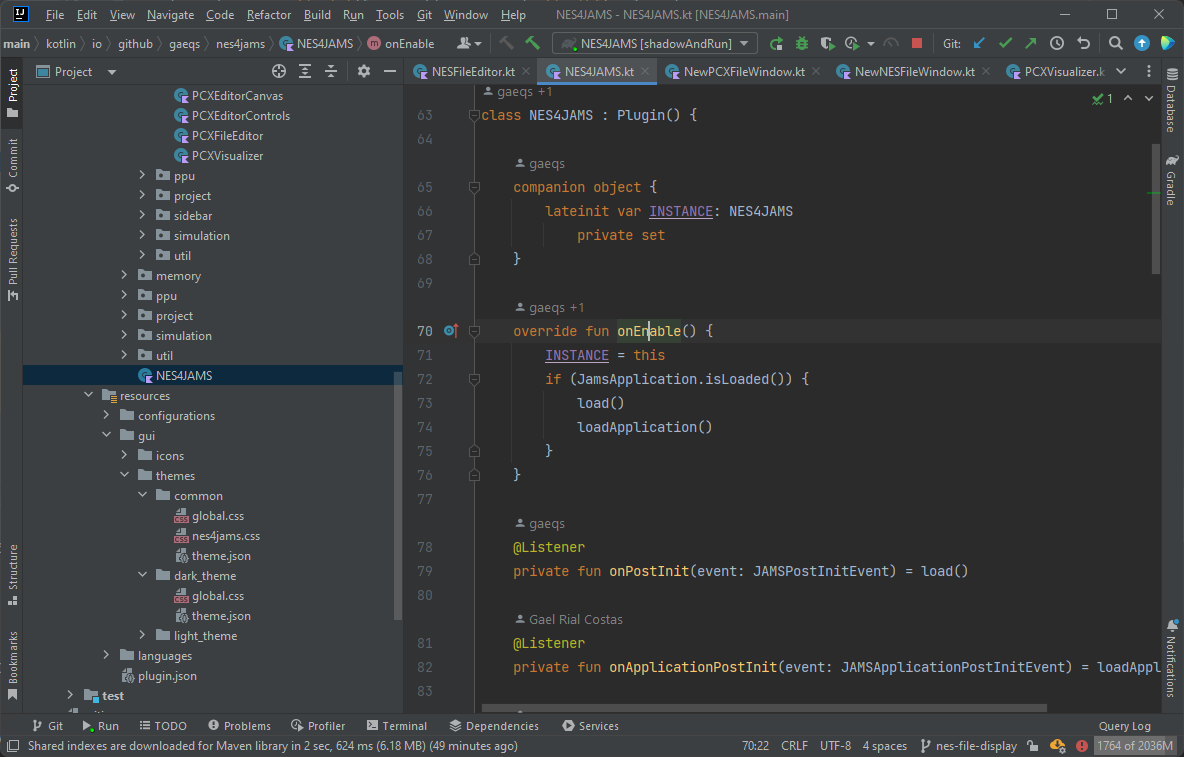
\includegraphics[width=0.8\textwidth]{images/result/idea-plugin}
    \caption{Desarrollo del componente \textit{NES4JAMS} en \textit{Kotlin}}
    \label{fig:jams-plugin}
\end{figure}

Gracias al uso de una versión de \textit{Java} moderna,
el desarrollo de la aplicación ha sido \textbf{mucho más rápido} y el resultado
ha sido \textbf{mucho más profesional}, pudiendo implementar diseños y
algoritmos rápidamente y con menores errores.
\textit{JavaFX} ha permitido desarrollar una interfaz de usuario
que se despega del conocido y desfasado formato de las aplicaciones
\textit{Swing}.
Gracias a su fácil desarrollo y su capacidad de usar código
\textit{CSS} para definir el estilo de la aplicación, \textit{JAMS}
puede presumir de tener un aspecto moderno y profesional.

Una de las ventajas que fue apareciendo durante el
desarrollo con respecto a utilizar \textit{Java} ha sido la
capacidad de poder usar otros lenguajes de programación capaces
de compilar a la \textit{JVM} para el desarrollo de componentes.
El desarrollador podrá escoger de un \textbf{amplio abanico de lenguajes}
de programación para el desarrollo de su componente.
Algunos ejemplos de lenguajes de programación que compilan a la \textit{JVM}
son \textit{Scala}, \textit{Kotlin} o \textit{Groovy}.
Un ejemplo de componente desarrollado en \textit{Kotlin} sería
\textit{NES4JAMS}, el cual es parte del Trabajo de Fin de Grado del Grado en
Diseño y Desarrollo de Videojuegos y cuyo método principal se puede observar
en la figura \ref{fig:jams-plugin}.


\section{Resultados relativos al objetivo 2}\label{sec:resultados-relativos-al-objetivo-2}

Los resultados de este objetivo corresponden a la creación de
un entorno base y un \textit{framework} que permita \textbf{implementar
diferentes entornos y herramientas}, creando así una capa
de abstracción que ayude a los desarrolladores y al propio
\textit{JAMS} a crear herramientas de manera rápida y sencilla.

Se considera que \textbf{se ha superado con creces}
el objetivo.
Gracias a las diferentes tecnologías que se han desarrollado
para la base, se pueden crear nuevas herramientas en cuestión
de minutos.
Los objetivos definidos en el Trabajo de Fin de Grado del Grado en
Diseño y Desarrollo de Videojuegos y mencionados en esta memoria
se han desarrollado paralelamente a este objetivo, resultando
en una aplicación base \textbf{robusta}, con capacidad de personalizar
una gran cantidad de aspectos del entorno.

La base también permite a los usuarios más comunes e
inexpertos personalizar el entorno de desarrollo gracias a la
\textbf{extensa configuración} y la capacidad de poder producir
\textbf{paquetes de idiomas y de temas}.
El resultado de estas personalizaciones se puede apreciar
perfectamente en la figura \ref{fig:jams-collage}.

\begin{figure}[h]
    \centering
    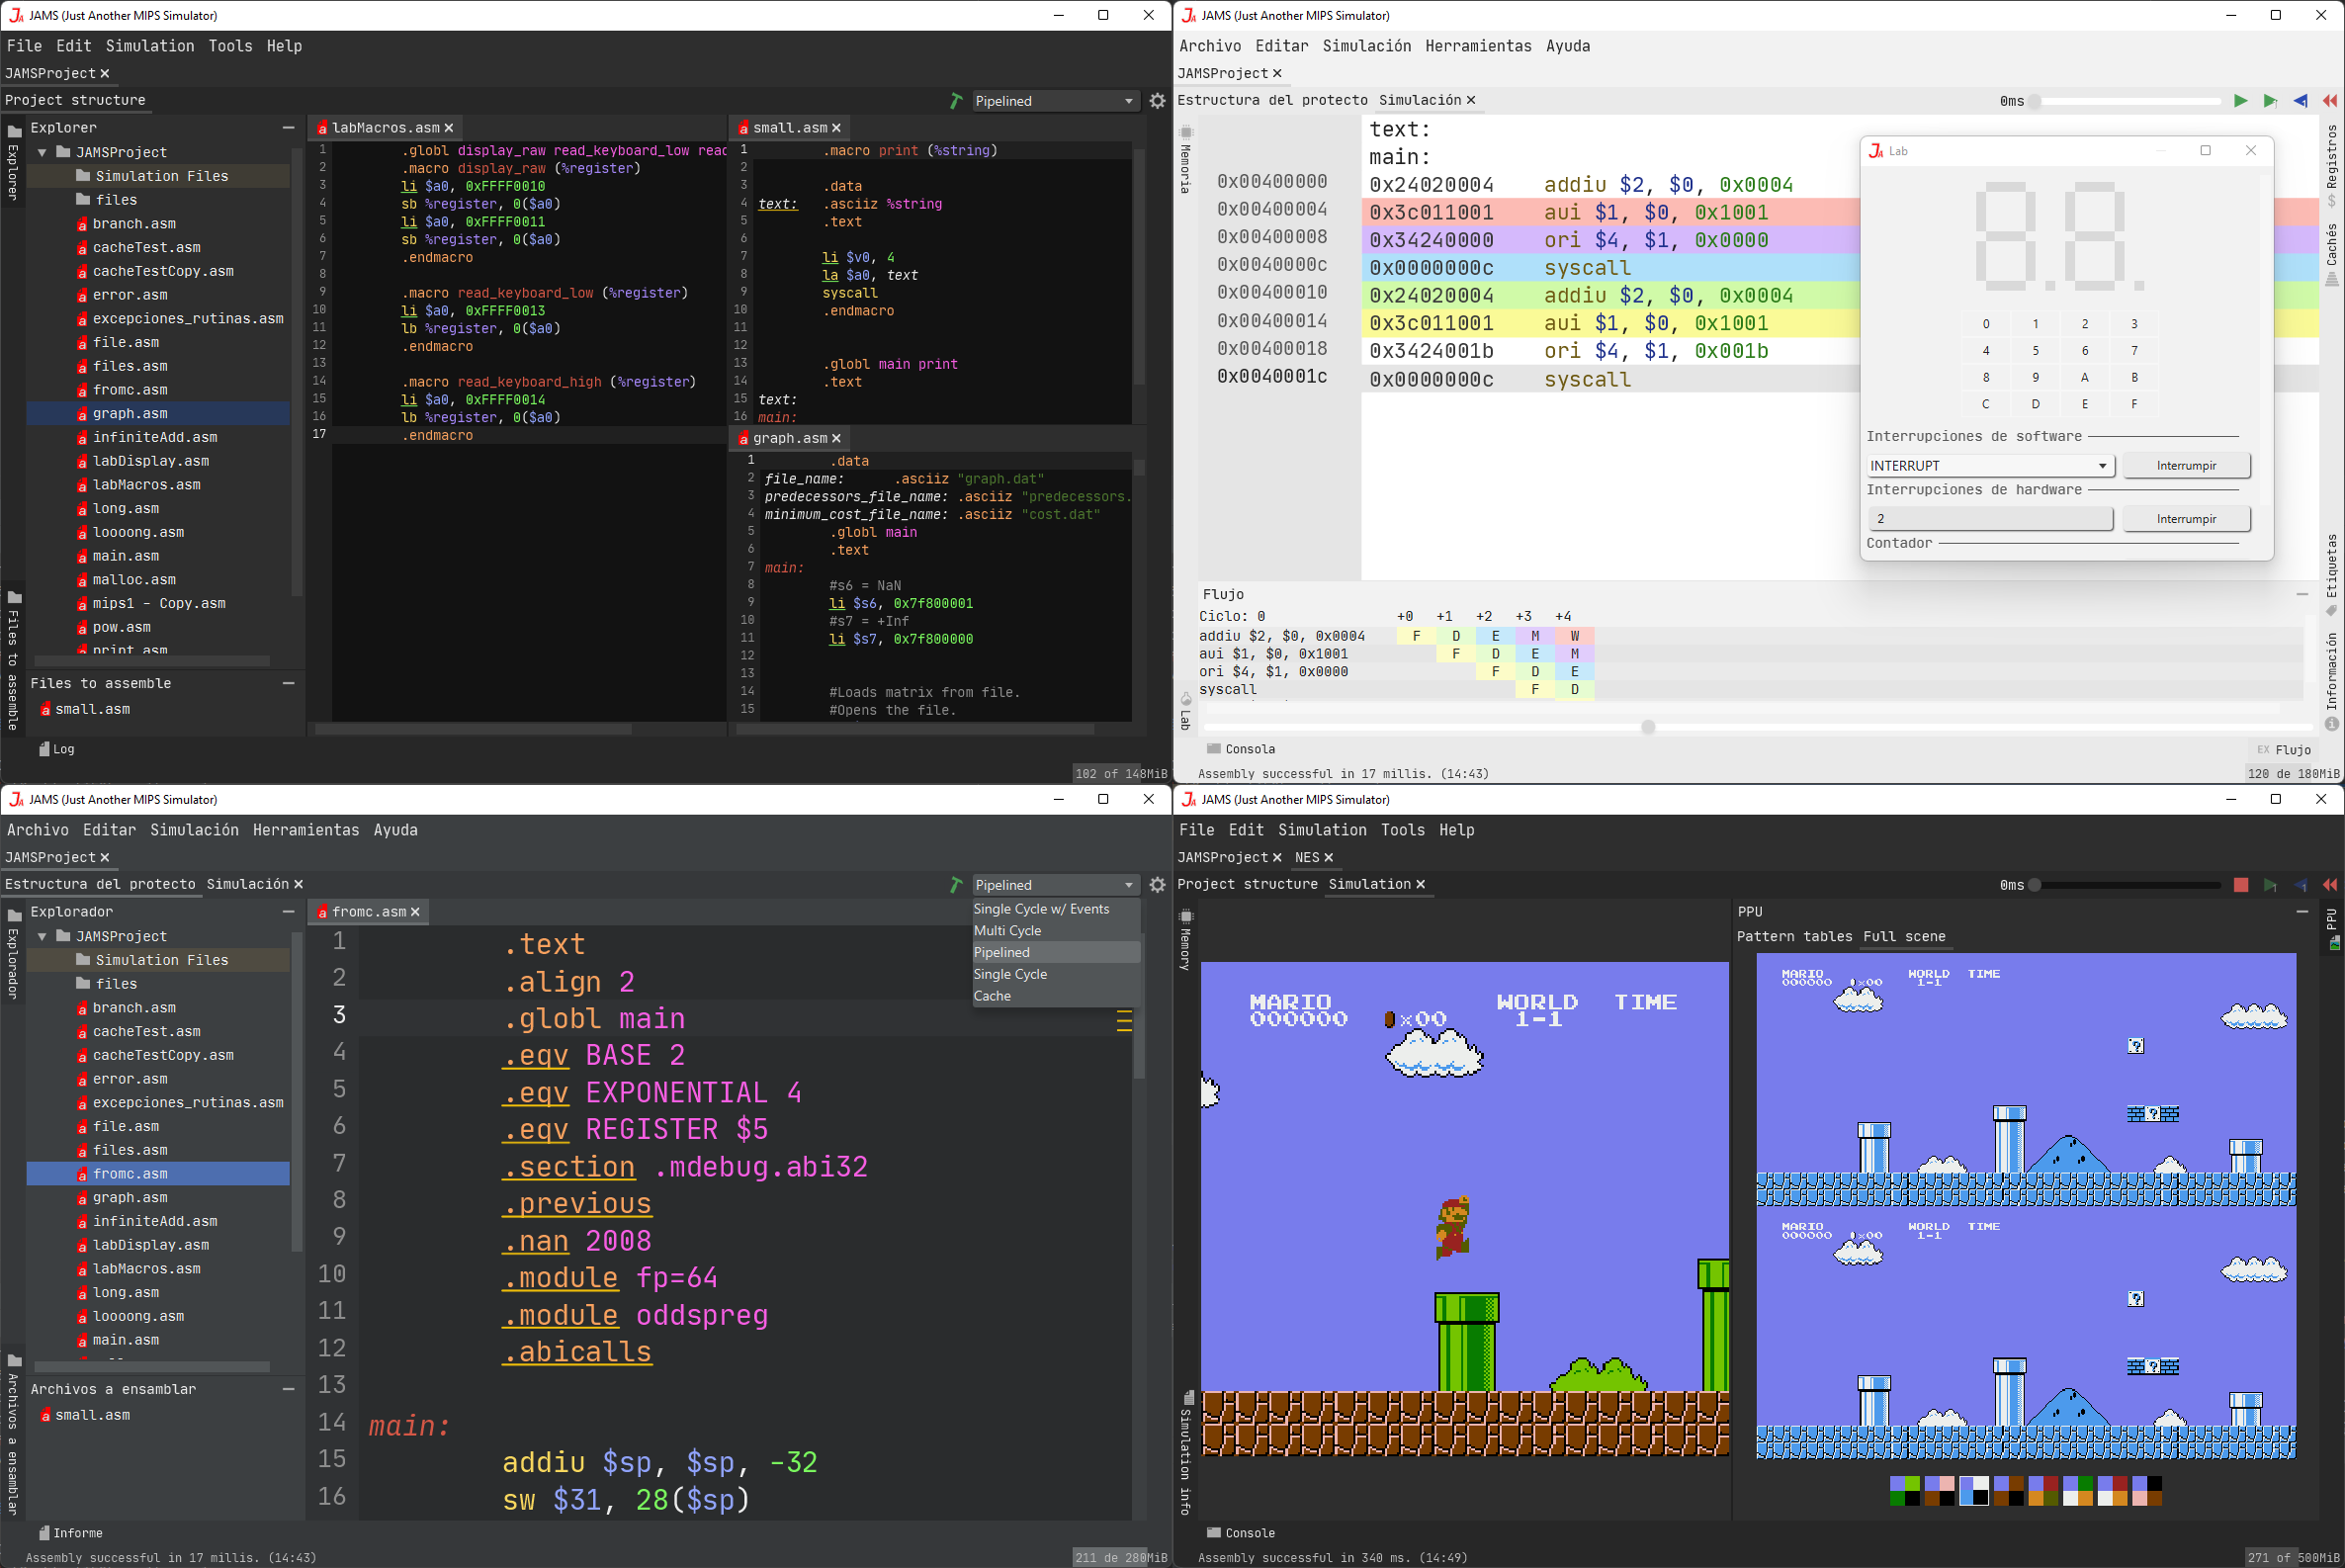
\includegraphics[width=0.8\textwidth]{images/result/jams-collage}
    \caption{Diferentes perfiles de personalización de JAMS}
    \label{fig:jams-collage}
\end{figure}

Por último, destacar el resultado de la \textit{interfaz de usuario}.
El uso de nodos como elemento central de la interfaz puede considerarse
un \textbf{acierto}: son componentes muy fáciles de usar y altamente personalizables.
Estos nodos son independientes entre sí, y muchos de ellos son \textbf{independientes}
de la tecnología que esté empleando el usuario, como es el caso del \textbf{explorador}.
Esto permite que sean herramientas \textbf{altamente reutilizables}, estando en todo
momento a disposición del desarrollador de componentes.


\section{Resultados relativos al objetivo 3}\label{sec:resultados-relativos-al-objetivo-3}

Los resultados de este objetivo corresponden al desarrollo
de un entorno de desarrollo para la arquitectura \textit{MIPS32}
usando la base creada en el objetivo anterior.
El objetivo requiere de la creación de un editor, un ensamblador
y un simulador, además de diferentes herramientas que complementen
a estos tres elementos principales.

Se considera que este objetivo se ha superado
de manera óptima.
\textit{JAMS} presenta de base un entorno de desarrollo completo
para la arquitectura \textit{MIPS32}.

El \textbf{editor de texto} está al nivel de los editores de texto
inteligentes que se pueden encontrar en los entornos de desarrollo
actuales, \textbf{ayudando al usuario} en la mayoría de las tareas
relacionadas con desarrollar una aplicación en ensamblador, como se observa
en la figura \ref{fig:mips-editor}.

\begin{figure}[h]
    \centering
    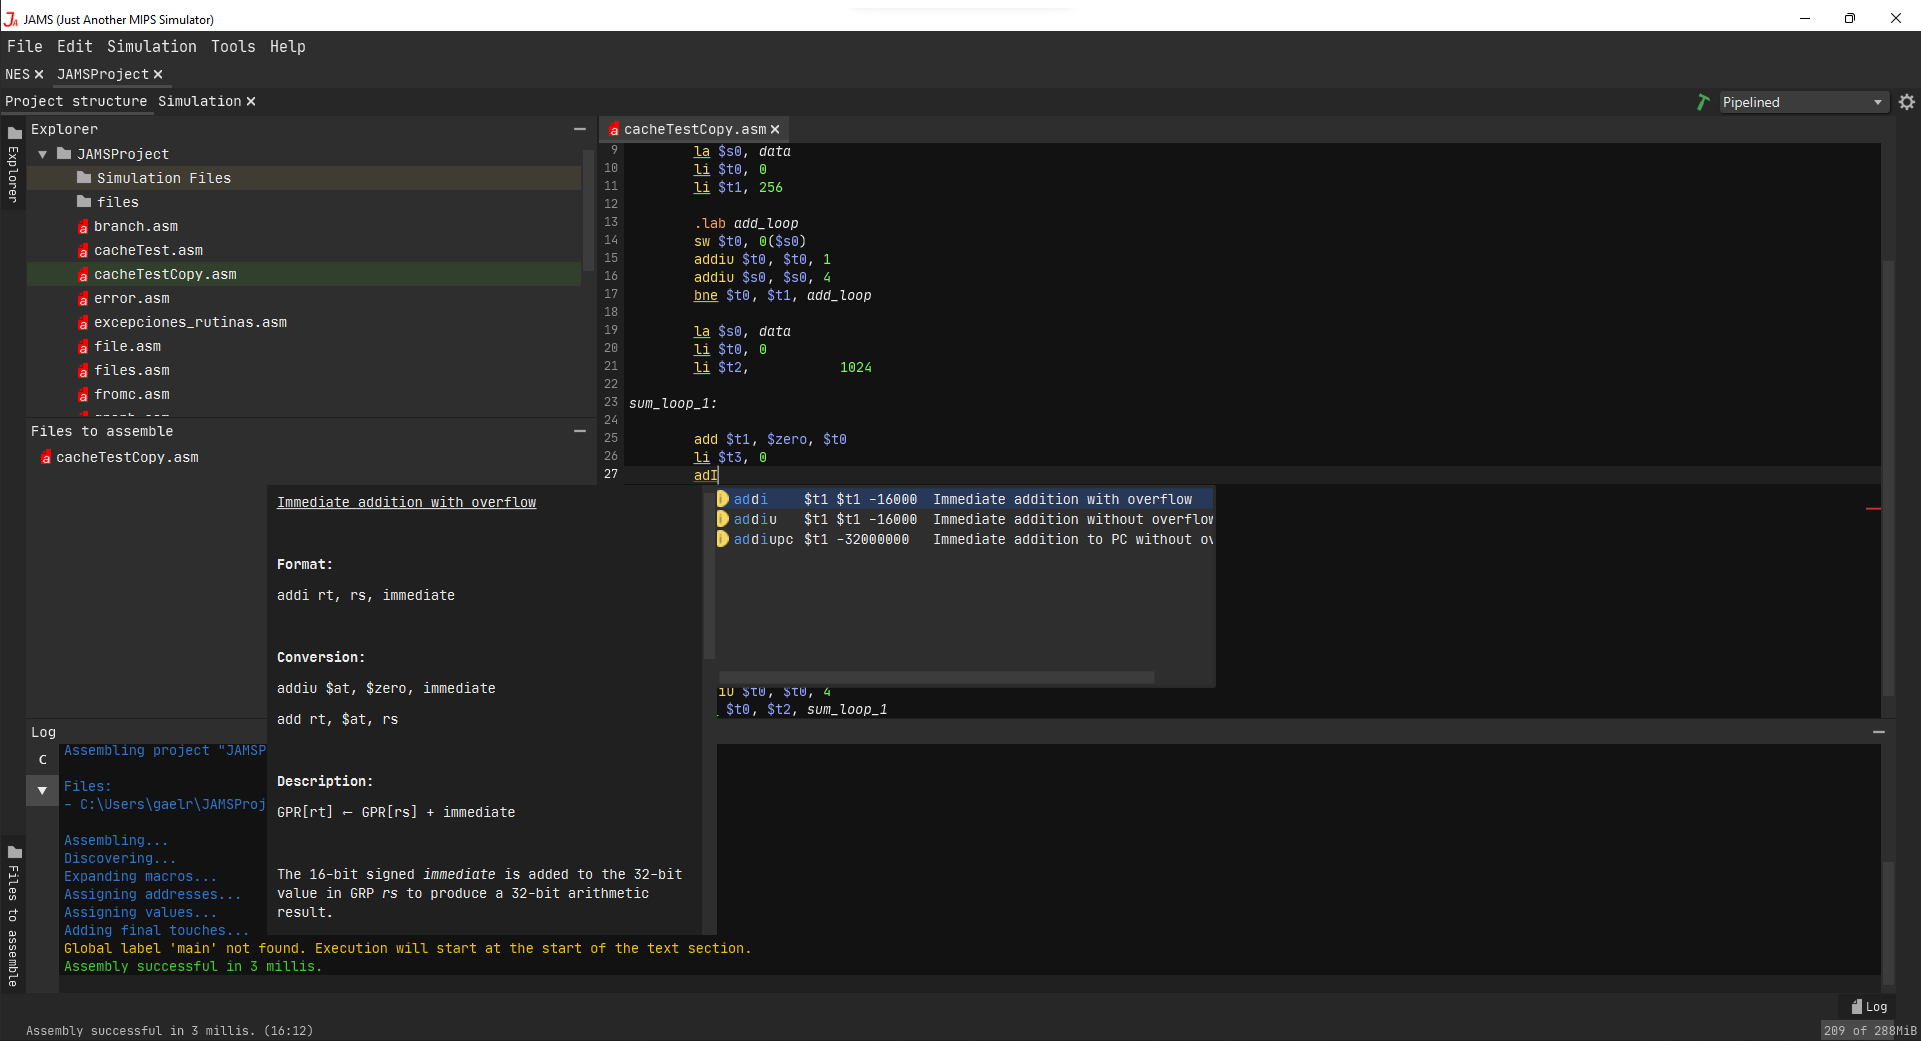
\includegraphics[width=\textwidth]{images/result/mips-editor}
    \caption{Editor de texto proporcionando ayuda al usuario}
    \label{fig:mips-editor}
\end{figure}

El \textbf{ensamblador} es altamente \textbf{personalizable},
permitiendo que otros componentes puedan aportar nuevas instrucciones y
directivas de manera sencilla.
Este ensamblador también incorpora varias \textbf{características avanzadas}
que el usuario puede usar, como son las \textbf{macros} y las
\textbf{etiquetas relativas}.

El \textbf{simulador} permite ejecutar código ensamblador
\textbf{MIPS32} en diferentes arquitecturas, siendo la arquitectura
uniciclo la más rápida de todas ellas, llegando a superar los
\textbf{40 millones de ciclos cada segundo}.
El simulador viene altamente equipado con diversas herramientas que
permiten al usuario \textbf{visualizar y modificar} el estado del simulador
de diversas maneras, tal y como se puede observar en la figura \ref{fig:mips-tools}.
Como detalle final, el simulador presenta una estructura basada en
\textbf{hilos}, lo que evita que la aplicación se congele al ejecutar
una aplicación.

\begin{figure}[h]
    \centering
    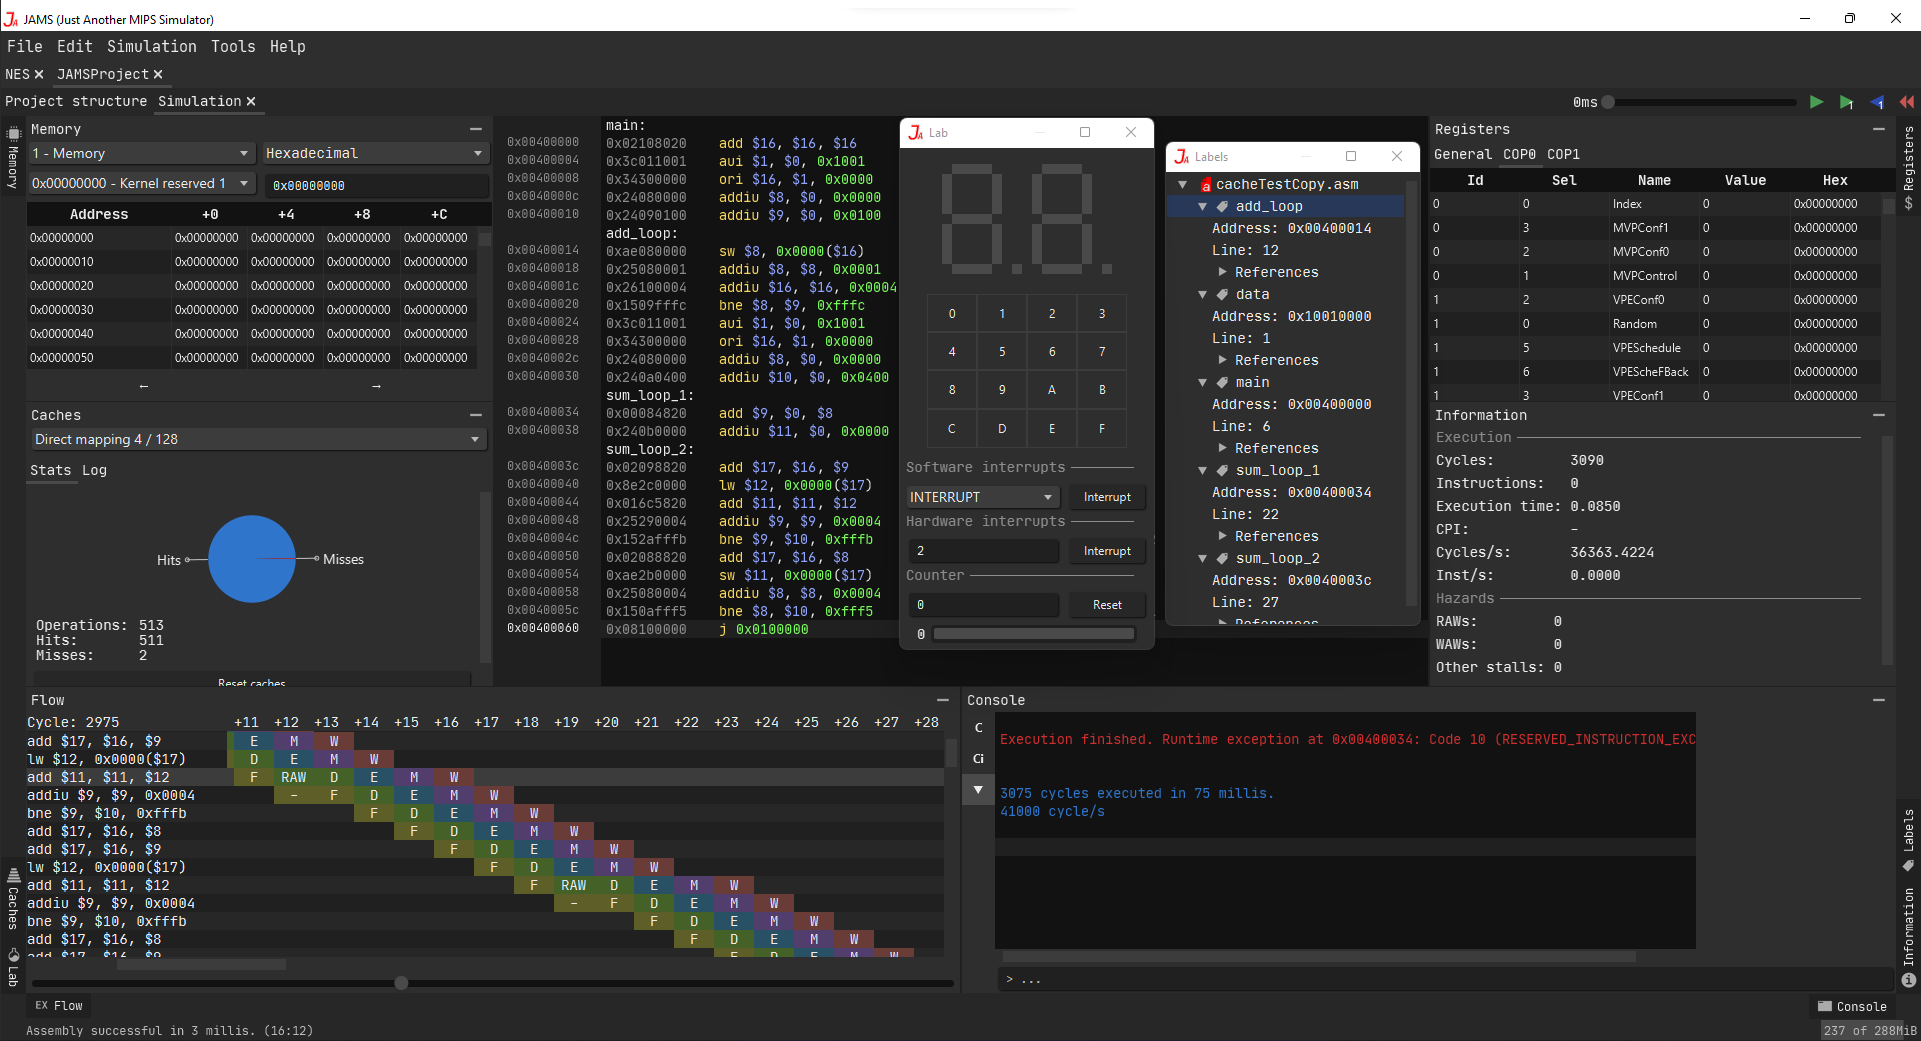
\includegraphics[width=\textwidth]{images/result/mips-tools}
    \caption{Todas las herramientas proporcionadas por el simulador}
    \label{fig:mips-tools}
\end{figure}